\documentclass{standalone}
% preamble: usepackage, etc.
\begin{document}

\chapter{强化学习基础}

强化学习是一种学习如何进行控制和决策的框架,强化学习的灵感来自于仿生学,它完成了从当前的环境状况到行为的映射,并通过学习这一映射过程使得从环境中得到的奖赏值最大化。这样一种框架被誉为可能是发展为强人工智能的框架,包括博弈论、控制理论、群体智能、多智能体系统等领域都与强化学习可以进行结合和交叉。在控制领域,强化学习被视为一种拟合动态规划方法。在博弈论领域,它被用来解释均衡点的出现及其原因。它和有监督学习,无监督学习组成了机器学习领域三个基本的学习框架。它不同于有监督学习和无监督学习,原因在于,在强化学习中,并不存在类似于有监督学习中的标签信息,只有奖赏信号用于指导整个学习过程,同样这也不同于无监督学习中没有任何信号和标签指导学习过程。\par

\section{智能体建模方法和马尔科夫决策过程}
强化学习框架的设计一般基于智能体建模的方式实现,基于智能体的模型是一种为了模拟控制和交互的计算模型,这样一种框架包括智能体和环境两类主体,其在多个领域都有广泛的应用,如在生物学中用于研究种群的分布,人口变化等问题,在经济和社会学中,用于研究城市人口流动和城市规划问题,消费者行为分析等。在强化学习中,我们通过图4-1所示的框架对强化学习进行建模。
\begin{figure}[h]
	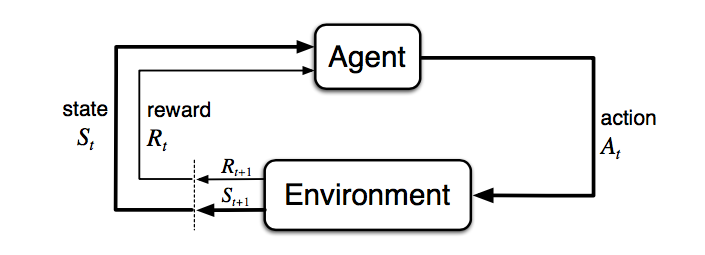
\includegraphics[width=12.0cm]{pic/4-1.png}
	\caption{强化学习框架}
	\label{4-1}
\end{figure}
\section{强化学习}

\subsection{价值函数}
\subsection{策略函数}
\subsection{基于价值函数的方法}
\subsubsection{查表法}
\subsubsection{函数近似法}

\subsection{基于策略梯度的方法}

\end{document}